%----------------------------------------------------------------------
\begin{frame}%[shrink]%[allowframebreaks]
  \frametitle{\KSe  \footfullcite{KurTsu75}$^,$\footfullcite{michsiv77}}


  \begin{equation}
    u_t+\frac{1}{2}(u^2)_x+u_{xx}+u_{xxxx}=0\,,\; x\in [0,L]
    \label{eq:ks}
  \end{equation}
  $u(x, t)$ represents the
  flame front velocity. $u(x, t) = u(x+L, t)$.

  \begin{columns}[c] % the "c" option specifies center vertical alignment
    %%%%%
    \column{.8\textwidth}
    \begin{itemize}
    \item {\color{blue} Galilean invariance}: \\
      $\ssp(x, t) \to \ssp(x-ct,t)+c$.

    \item {\color{blue} Reflection invariance}:  \\
      $R\,\ssp(x,t) = -\ssp(-x,t)$. \\
      %$a_k \to -a_k^{*}$ in the Fourier mode space.

    \item {\color{blue} Translation invariance}: \\
      $\LieEl(\gSpace) \ssp(x, t) = \ssp (x+\ell,t)$.
      Here $\gSpace = 2\pi \ell/L$.  \\
      %$a_k \to e^{iq_k\gSpace} a_k$ in this Fourier mode space
      %with $\gSpace = 2\pi \ell/L$.
    \end{itemize}

    %%%%%
    \column{.2\textwidth}

    \begin{center}
      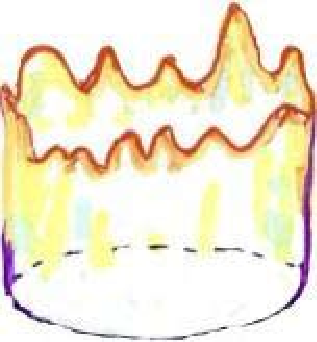
\includegraphics[width=1\textwidth]{flameFlut-fig}
    \end{center}

  \end{columns}

  \begin{center}
    {\color{green}  Reduce Galilean invariance : set $\int dx\, u = 0$. }
  \end{center}

  % \note[item]<1>{
  %   $\int dx\, u$ represents the mean velocity.
  % }


\end{frame}

%======================================================================
\subsection{Invariant solutions}

%----------------------------------------------------------------------
\begin{frame}[shrink]%[allowframebreaks]
  \frametitle{Invariant solutions : \eqva}
  \putsym

  \htb{Defintion: $\ssp(\zeit) = \ssp(0)$,\quad \ie, $\vel(\ssp) = 0$}

  \begin{center}
    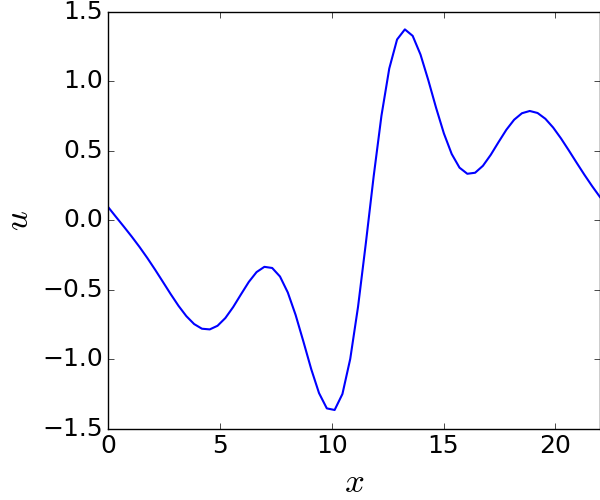
\includegraphics[width=0.32\textwidth]{ksEq1}
    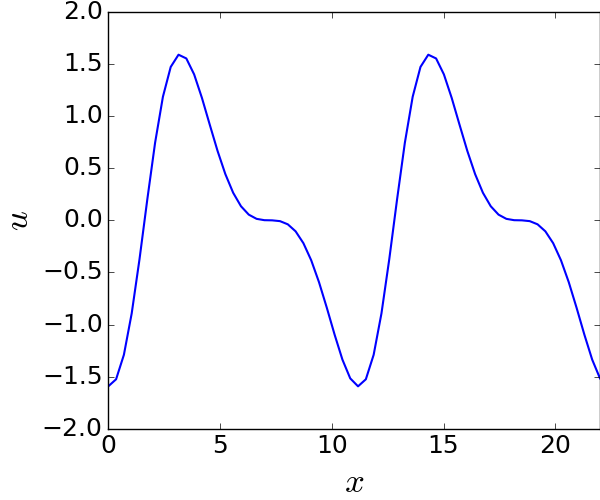
\includegraphics[width=0.32\textwidth]{ksEq2}
    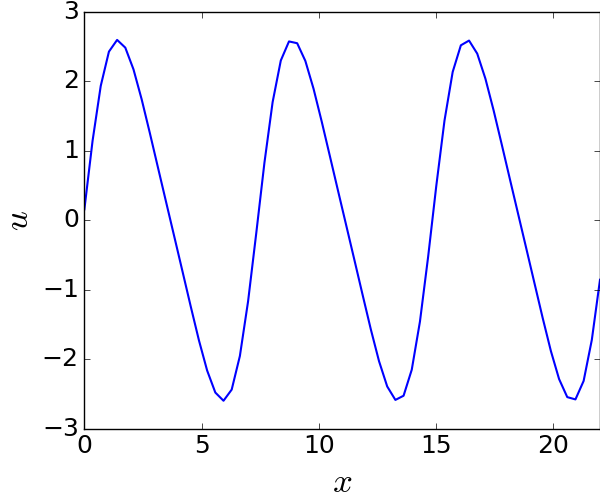
\includegraphics[width=0.32\textwidth]{ksEq3}

    {
      Three \eqva: (a) \EQV{1}, (b) \EQV{2}, and (c) \EQV{3}
    }
    %\label{fig:kseq}
  \end{center}

\end{frame}

%----------------------------------------------------------------------
\begin{frame}[shrink]%[allowframebreaks]
  \frametitle{Invariant solutions: \reqva}
  \putsym

  \htb{Defintion:
    $\ssp(t) = \LieEl(t \, \velRel) \, \ssp(0)$
  }
  (also called \emph{traveling waves})

    \begin{center}
    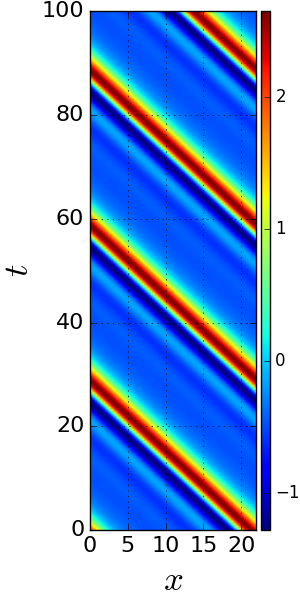
\includegraphics[width=0.2\textwidth]{ksReq1T100}
    % (b)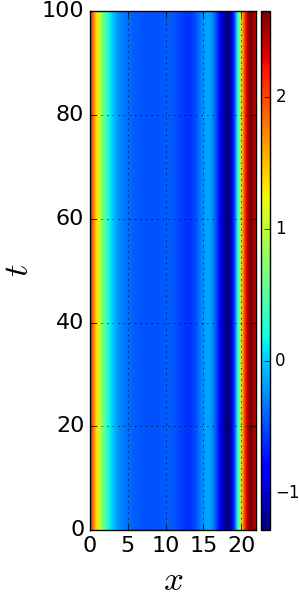
\includegraphics[width=0.2\textwidth]{ksReq1T100Red}
    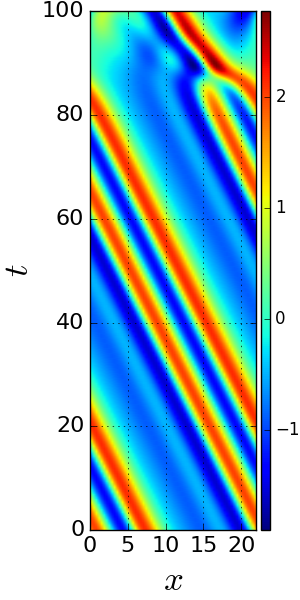
\includegraphics[width=0.2\textwidth]{ksReq2T100}
    %(d)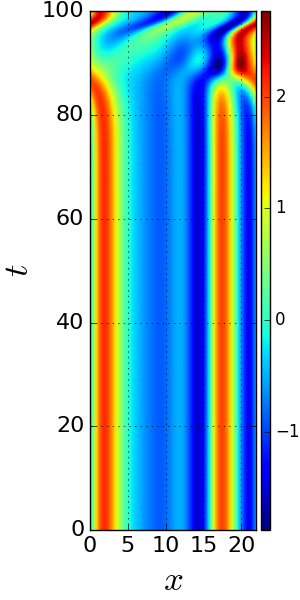
\includegraphics[width=0.2\textwidth]{ksReq2T100Red}
    %\caption[\Reqva\ in the full \statesp\ and in the slice in the one-dimensional \KSe.]

    {
      Four \reqva: \REQV{+}{1}; \REQV{+}{2}; and their reflections
    }
    \end{center}
    %\label{fig:ksreqT100}

\end{frame}

% ----------------------------------------------------------------------
\begin{frame}[shrink]%[allowframebreaks]
  \frametitle{\small Invariant solutions: pre\po s and \rpo s}
  \putsym

  \htb{
    pre\po : $\ssp(0)=R\ssp(\period{p})$

    \medskip
    \rpo : $\ssp(0)=\LieEl_p\ssp(\period{p})$, with $\LieEl_p=\LieEl(\gSpace_p)$
  }

    \begin{center}
    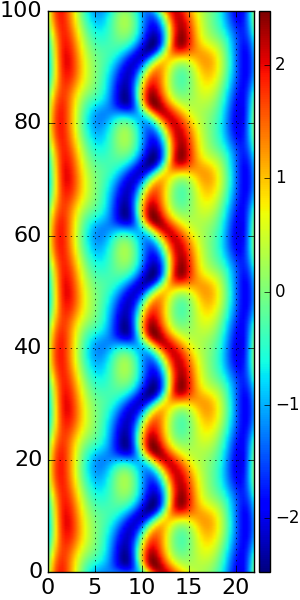
\includegraphics[width=0.16\textwidth]{ksppo1T100NoLabel}
    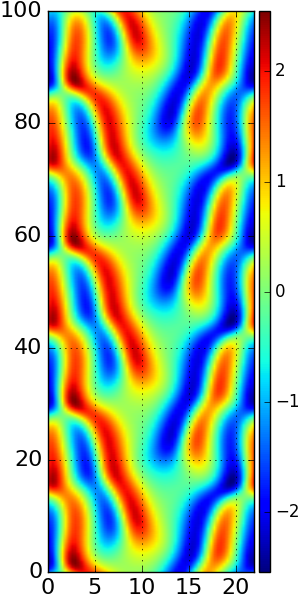
\includegraphics[width=0.16\textwidth]{ksppo2T100NoLabel}
    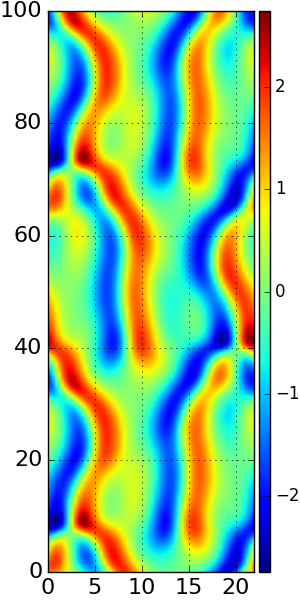
\includegraphics[width=0.16\textwidth]{ksppo3T100NoLabel}
    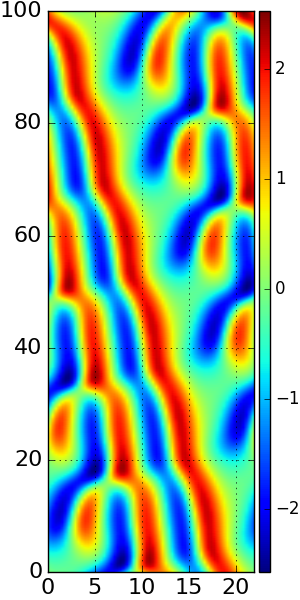
\includegraphics[width=0.16\textwidth]{ksrpo1T100NoLabel}
    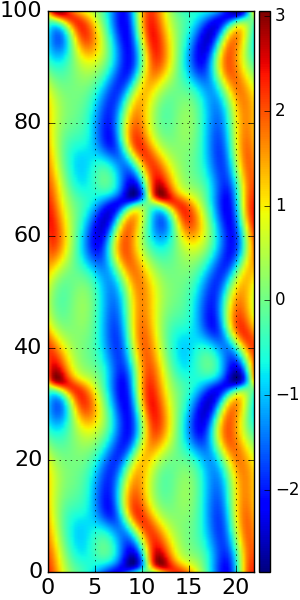
\includegraphics[width=0.16\textwidth]{ksrpo2T100NoLabel}
    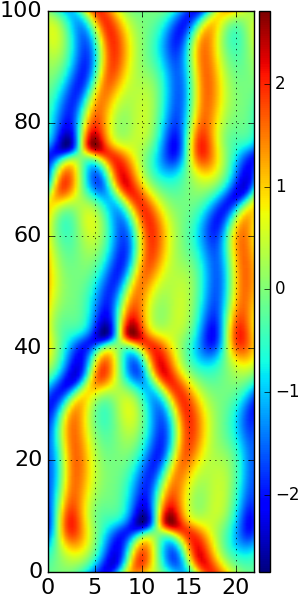
\includegraphics[width=0.16\textwidth]{ksrpo3T100NoLabel}
%    \caption[Pre\po s and \rpo s in the full \statesp.]

    {
      Left three: \PPO{10.25}, \PPO{14.33} and \PPO{32.36}

      Right three: \RPO{16.31}, \RPO{32.80} and \RPO{33.50}
    }
    \end{center}
    %\label{fig:kspoT100}
\end{frame}

% ----------------------------------------------------------------------
\begin{frame}[shrink]%[allowframebreaks]
  \frametitle{\Statesp}
  \putsym

  \begin{center}
    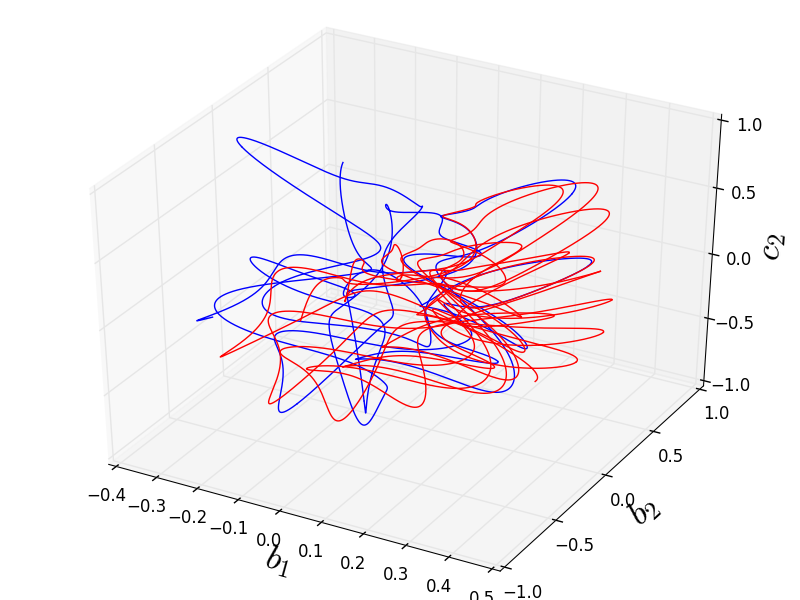
\includegraphics[width=0.6\textwidth]{ksrpo5rpo22}

    {
      \htb{\RPO{35.97}} and \htr{\RPO{57.59}}.
    }
  \end{center}
  \htb{
    Fourier mode : $a_{k}=b_{k}+ic_{k}$. \\
    \statesp:
    $\cssp=(b_{1},c_{1},b_{2},c_{2},\cdots,b_{N/2-1},c_{N/2-1})^\top$.
  }

\end{frame}

% ----------------------------------------------------------------------
\begin{frame}[shrink]%[allowframebreaks]
  \frametitle{\SOn{2}-reduced state space}
  \putsym

  \begin{center}
    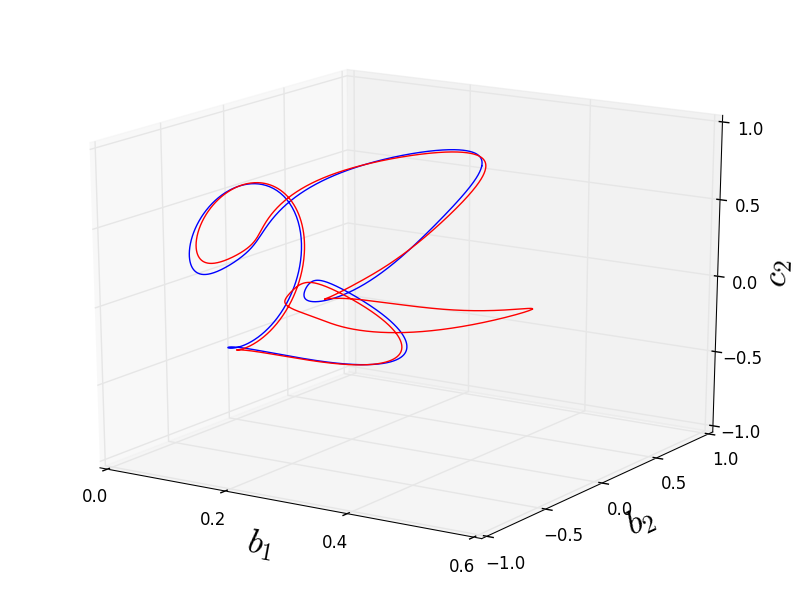
\includegraphics[width=0.7\textwidth]{ksrpo5rpo22red}

{
      \htb{\RPO{35.97}} and \htr{\RPO{57.59}}.
    }
  \end{center}

\end{frame}
